\chapter{UX Design Cycle 2}
\label{ch:ux2-cycle_report}

The User Experience Design Cycle 2 plan and results discussed here. \\

As significant improvisation over the previous user experience design cycle, we improved the codebase as with number of bug findings shown on user interface. Also, the number of tools shown as integrated is ten while in the previous cycle, we shown only two. This enhancement helps to test whether the previous solution ideas still hold in terms of scalability. Besides, we evaluate solutions ideas corresponding to code view while in previous cycle only analysis view is investigated. \\

\section{Research Questions}

This section shows the list of sub research questions considered for each main research question. In the case of the first primary research question, i.e., with displaying results for a single project from multiple static analysis tools, the following are the sub research questions. \\

\begin{enumerate}
\item From analysis view perspective, does a separate list or single list help the user to identify the common bug?
\item From analysis view perspective, will tags help in scalability of bug results in comparison to separate list or single list?
\item From code view perspective, will single icon suffice the showing of different tools icons?
\end{enumerate} 

Next, in the case of the second main research question, i.e., with feedback while bug fixing is on-going, the following are the sub research questions. \\

\begin{enumerate}
\item When submitting the bug for analysis, what feedback does user feel convenient among animation, progress bar or popup?
\item Does a single type of feedback suffice or requires combination?
\item From code view perspective, i.e., once user fixed a bug and submitted for analysis and then off the analysis results screen, then is popup notifications with analysis progress information better to busy status (spinner)?
\end{enumerate} 


Finally, in the case of the third main research question, i.e., with carrying traceability of bug fixing, the following are the sub research questions. \\

\begin{enumerate}
\item In tracing, will the user need to know the changes made to fix a bug affecting the analysis of other tools?
\item Does adjective mapping ease the user to trace the changes made in code in terms of bugs existence?
\item From code view perspective, will the bug tool icons with before/after code help understand the user in easing to fix it?
\end{enumerate} 

\section{User Study Process and Results}

This section explains the user scenario and questionnaire used during the user study.

\subsection{Metrics Analysed}

\subsubsection{Quantitative measurements}  

\begin{enumerate}
	\item Task Success: Whether the user able to complete the respective task or not?
	\item For each research question, ask users to evaluate the solution idea in terms of perceived usability on a Uni-polar Likert scale of 0-10. Scale: 0 – worst, 10 – best, in comparison to alternative solution idea provided.
\end{enumerate} 

\subsubsection{Qualitative measurements} 

Usability: Ask the user to provide feedback through cognitive walkthrough process about problems faced while using the prototype and get insights about the solution idea. \\

\subsection{User Study}

\subsubsection{Pre-test}

By first, the user background is verified with the pre-test questionnaire whether he/she is the right candidate to consider for user study. The ideal choice is the user who has Computer Science studies background and programs software projects. Also, we examine whether the user has used any static analysis tools and if so, the relationship between their favourite tool and usability is found out. \\

Questionnaire: \\

\begin{enumerate}
\item How often does the user do software development (i.e., coding)?
\item Have the user used static analysis tools?
\item What tools have the user used?
\item Is it IDE integrated tool or any other dedicated tools such as FindBugs, PMD.
\item Which is the user’s favourite one? 
\item Why is it favourite? Any correlation to its better user interface feature? \\
\end{enumerate}

\textbf{Results}: \\

There are seven users participated in this user study phase. Everyone has Computer Science background with at least a bachelor’s degree, and also, three users have sound professional experience. Among them, six users are pursuing master’s degree in computer science at the time of this user study and one user is a research assistant in the research group Software Engineering.  \\ \\

Out of 7 users, three users almost do coding on every day, and remaining users on an average do coding three days in a week.  Only one user used static analysis tools and a core developer of one of his static analysis tools and. In contrast, remaining users usually do manual testing or use debugger in order to find any bugs in their code. Nevertheless, all users are familiar or at least heard of static analysis in general. One user used tools namely SpotBugs, FindSectBugs and his tool titled CogniCrypt, which can integrate into IDE called Eclipse. Among them apart from his tool. SpotBugs was his favourite one. The reason is that he likes its functionality by how fast it is and also the presentation of bug findings is ok. With regards to the importance of user interface in addition to functionality, users felt the importance should be given for both as they both matter and interface would be beautiful to have for better visualisation of existence of bugs. One user said that he uses Visual Studio IDE, which is intuitive and easy to use, thereby expects to be able to have such interface familiarity with static analysis tools. One user expressed that this research work is stepping in the right direction. It is encouraging to hear from a user who is having a lot of programming experience about ten years. One user mentions that more tools it reports a particular bug then it ensures the finding is a bug. This thinking is again interesting to hear as it inlines the purpose of this thesis. \\ \\ 

Once we do the pre-test questionnaire, the user is asked to assume that they are working on a software project and want to find bugs in their codebase. There are ten tools linked to their codebase for better coverage of vulnerabilities. Next, walk through three main research questions concerning its user interface one by one with their sub research questions and evaluate their solution ideas for both analysis view and code view. \\ \\

Prototypes are made based on solution ideas, i.e., wireframes using Balsamiq software tool. They are presented to user one after other in random order. Then a cognitive walkthrough is carried out with think-aloud process during user study. \\ \\

Now let us walk through each research question. \\ \\

\subsubsection{RQ 1: How to display the results of the same codebase from different analysis tools?}

As part of this research question, there are three sub research questions considered. We made the solution ideas for analysis view such as single list, separate list and tags into respective prototypes, and for code view, the ideas are single icon and separate icons. Then we evaluate the solution ideas with the following pattern with User Scenario. Task and Follow up questionnaire. We consider a success criteria to the task in order to determine whether the user can perform the task or not on the presented prototype of respective solution idea. Once we present the three solution ideas for analysis view, we ask the follow-up questions. \\ \\

\textbf{User Scenario}: \\

The following user scenario is presented to the user, “Assume you as a Software Developer working on a project and about to see the analysis results in a given user interface.” \\ \\

\textbf{Task}: \\

Understand the results and Identify the common bug reported by tools. \\ \\

\textbf{Follow Up}: \\

\begin{enumerate}
\item Do the user desire to have “union” or “intersection” results when selecting multiple tools through filter? 
\item Among the solution ideas presented, which one do gentle feel convenient (easy to use) with for the given task?
\item Why is it the mentioned solution idea is convenient?
\item How do the user rate in terms of perceived usability ranging from O be lower to 10 be high for provided solution designs in comparison?
\item Which UI does the user think scales better with increase in bugs? \\
\end{enumerate}

Now let us begin with first solution idea to analysis view, i.e., Single list. \\

\textbf{Solution Idea: ( Single List )} \\

As we know, each static analysis tool has a respective name and an icon representing it. So, when we integrate multiple tools, we either must use tool names or icons to represent the respective analysis tool while displaying the bug-finding results that indicates which bug was identified by what tool. In the current scenario, an idea of having a table view with a tool column that shows tool icons for a respective bug finding. This idea could be well understood, looking at following  \autoref{fig:S21_single_list} or a complete prototype images added in appendix. \\ \\


\begin{figure}[hbt!]
	\centering
	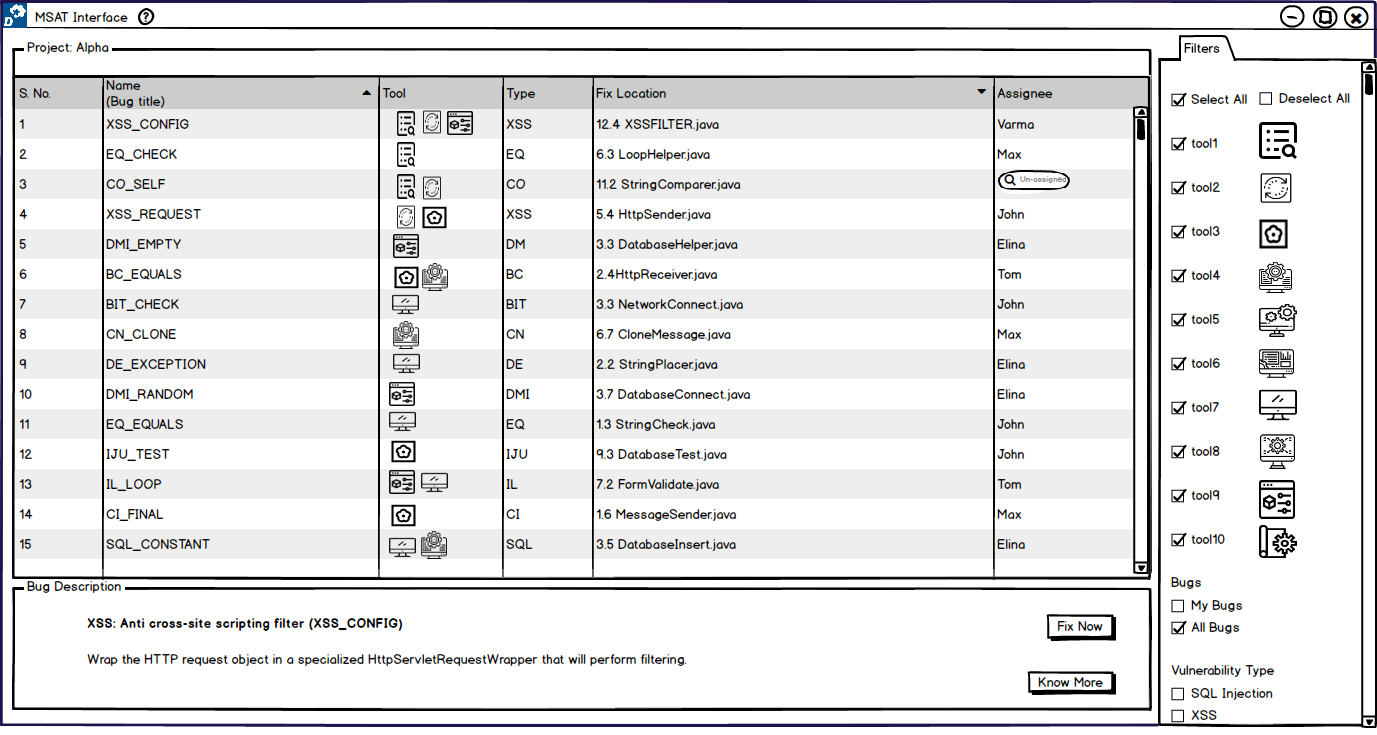
\includegraphics[width=\linewidth]{figures/solution_ideas_snaps/S21_single_list}
	\caption{An interface prototype showing ‘single list’ solution idea.}
	\label{fig:S21_single_list}
\end{figure} 

\textbf{Task – Success Criteria}: \\

User finds the “Bug name – XSS\_CONFIG” which is a common bug by clicking on ‘Select all’ tools filter. \\

Also, the user interface is demonstrated by showing multiple screens for each tool and the significance of an icon. This added demonstration is to ensure the user gets the solution idea. \\ \\

\textbf{Evaluation}: \\

Quantitative Results: \\

There are seven user study participants. Among them, five users manage to perform the task, and the remaining two users could not do so. This evaluation shows that the task success rate is 71.43 per cent. \\

Among the seven users, five users felt this is convenient in considering a final solution idea in showing the analysis results, in comparison to other solution ideas. In terms of usability on a scale of 0 to 10, where 0 being the worst and ten being the best, seven users rated the solution idea in comparison to alternate solution ideas i.e., separate list and tags as 7,6,7,10,9,9 and 9, which averages to 8.14. \\

Qualitative Results: \\

Let us now investigate the reasoning behind the user’s choice of solution idea and respective ratings. The reasoning behind the low task success rate is because one user expected to see intersection of results with tool selection. So, got lost in that thinking as in present prototype it shows union of bug findings by the selected tools in filter and other user understood the task differently, i.e., finding the same kind of bug identified by the tools.  Users felt that selecting tools shows common bugs, and got used to represent data in tables. It is effortless to perceive, more user-friendly, icons are always gentle relief to eye; it scales better, much better to understand and also much convenient. Two users have mentioned about their expectation that selections of tools results in only common bug-findings as results. Also, three users mentioned the presentation of tool icons and their names. One user suggested to use tool names instead of icons in case where they are not so distinctive. Similarly, one user stated that it could confuse to relate which icon represents what tool. As an improvement, there is a suggestion from different user to have tool names that appear on scroll over tool icon. \\

\textbf{Solution Idea: ( Separate List )} \\

Similar to the previous one, now the idea is showing separate table view for each tool. This idea could be well understood, looking at following \autoref{fig:S21_seperate_lists} or a complete prototype images added in appendix.  \\


\begin{figure}[hbt!]
	\centering
	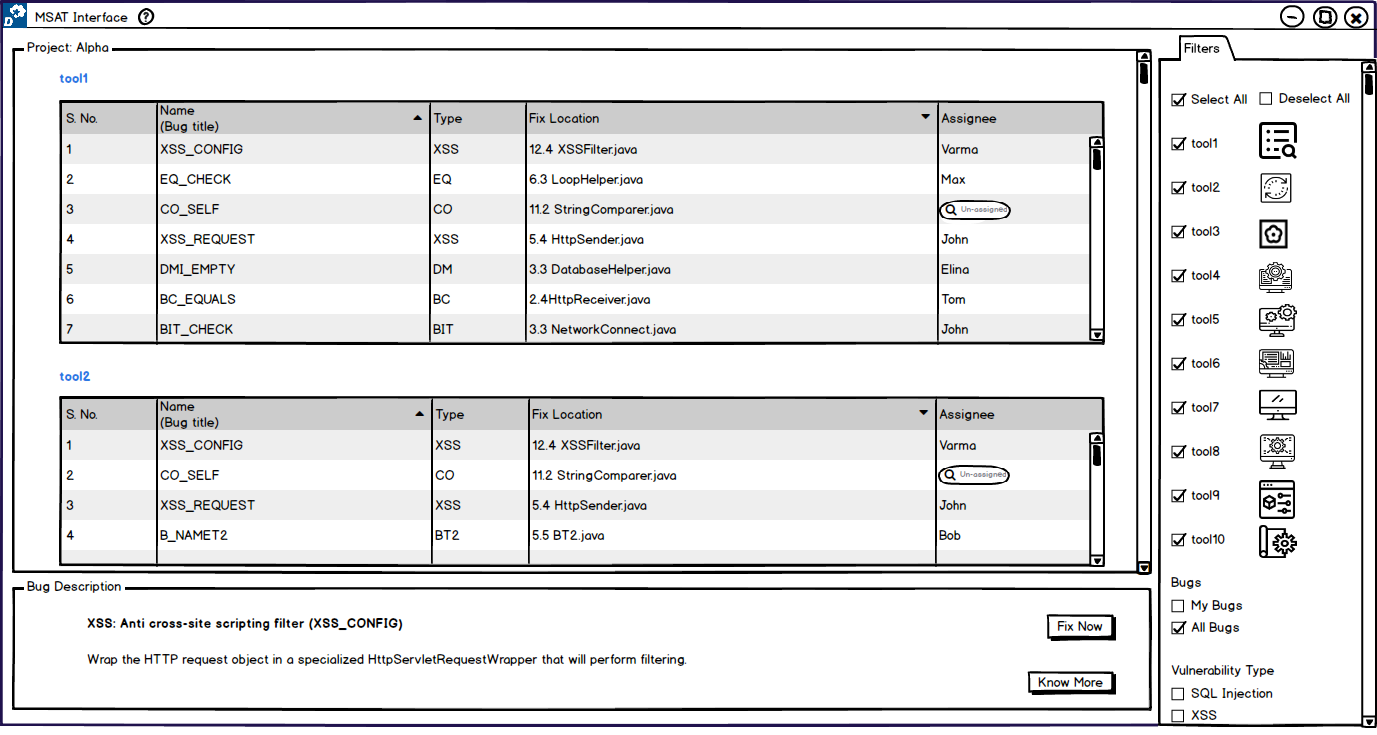
\includegraphics[width=\linewidth]{figures/solution_ideas_snaps/S21_seperate_lists}
	\caption{An interface prototype showing ‘seperate lists’ solution idea.}
	\label{fig:S21_seperate_lists}
\end{figure}

\textbf{Task – Success Criteria}: \\

User scrolls to see the results until tool six and find the Bug name – XSS\_CONFIG, which is a common bug. \\

The user can scroll until tool six only as it signifies the real-time scenario where sometimes tool 7, 8. 9 and 10 does not report any bugs. Also, the user interface is demonstrated by showing the bugs related to different tools separately and the bugs related to tool one and tool 3. \\
\clearpage
\textbf{Evaluation}: \\

Quantitative Results: \\

There are seven user study participants. Among them, only three users manage to perform the task, and the remaining users could not do so. This evaluation shows that the task success rate is 42.85 per cent. \\

Among the seven users, no user felt this is convenient in considering a final solution idea in showing the analysis results, in comparison to other solution ideas. In terms of usability on a scale of 0 to 10, where 0 being the worst and ten being the best, seven users rated the solution idea in comparison to alternate solution ideas i.e., single list and tags as 3,6,5,7,6,7 and 4, which averages to 5.43. \\

Qualitative Results: \\

Let us now investigate the reasoning behind the user’s choice of solution idea and respective ratings. The reasoning behind the low task success rate is because one user expected to see intersection of results with multiple tools selection. So, it made him lost in thinking, and one user felt it is not the best UI to do the task, so dropped off, and two users felt it is time-consuming. Also, some users felt there is no enough space to analyse and especially challenging to identify the common bug correctly. In contrast, there is one user who felt that this solution idea makes it more comfortable to perceive. \\

\begin{myboxi}{{\textbf{RQ 1-1: From analysis view perspective, does a separate list or single list help the user to identify the common bug?}}}
\\ \\	Users preferred single list as it is more user-friendly and effortless to perceive.
\end{myboxi}	
	
\textbf{Solution Idea: ( Tags )} \\

As we have seen so far using icons for representing an analysis tool. Now, having a tag name for each tool and used for bug finding results displayed in a complete list view. StackOverflow user interface inspires the present solution idea. This approach could be well understood, looking at following \autoref{fig:S21_tags} or a complete prototype images added in appendix.  \\



\begin{figure}[hbt!]
	\centering
	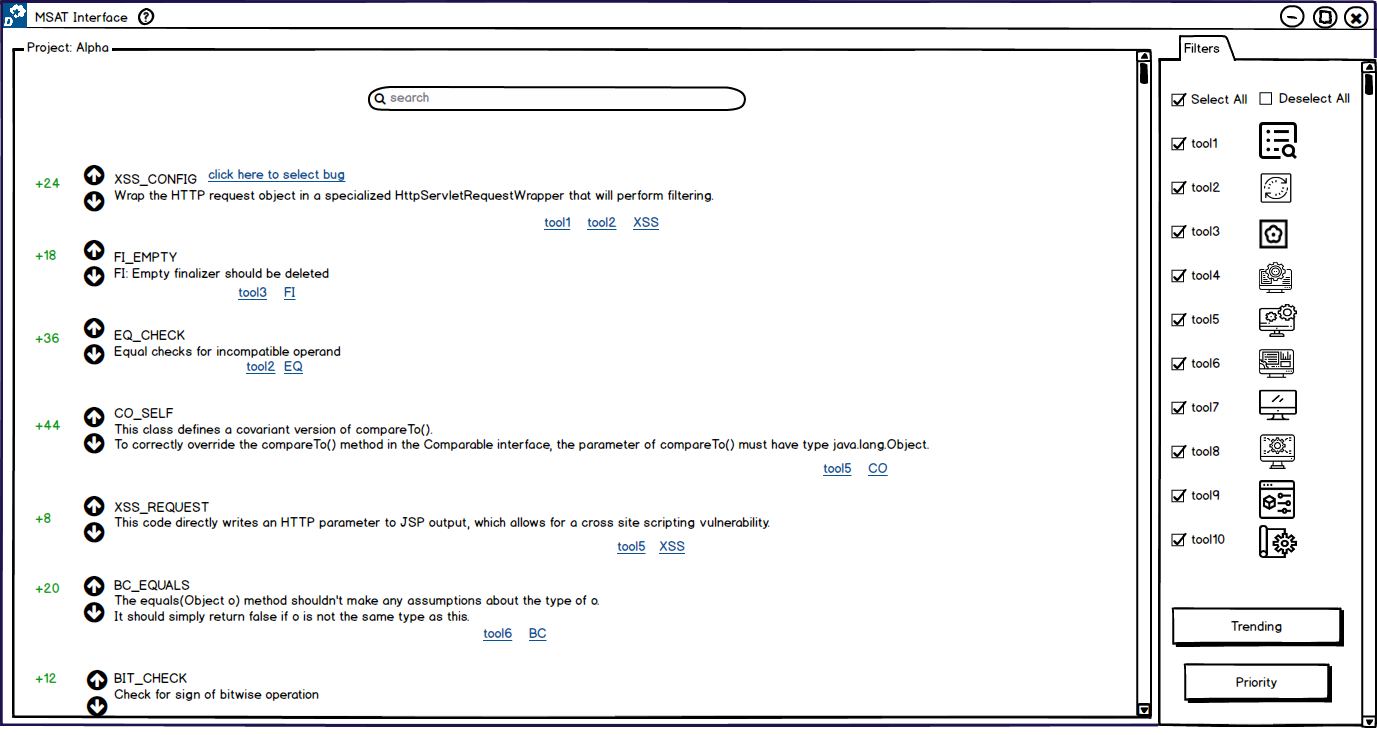
\includegraphics[width=\linewidth]{figures/solution_ideas_snaps/S21_tags}
	\caption{An interface prototype showing ‘tags’ solution idea.}
	\label{fig:S21_tags}
\end{figure}


\textbf{Task – Success Criteria}: \\

User scrolls down three screens to see the results and find the Bug name – XSS\_CONFIG, which is a common bug. \\

Also, the user interface is demonstrated by showing alternative approaches to see bugs reported by tool1. \\

\textbf{Evaluation}: \\

Quantitative Results: \\ \\
There are seven user study participants. Among them, six users managed to perform the task. This evaluation shows that the task success rate is 85.71 per cent. Among the seven users, two users felt this is convenient in considering a final solution idea in showing the analysis results, in comparison to other solution ideas. In terms of usability on a scale of 0 to 10, where 0 being the worst and ten being the best, seven users rated the solution idea in comparison to alternate solution ideas i.e., single list and separate list as 8,7,6,8,7,9, and 6, which averages to 7.28. \\

Qualitative Results: \\

Let us now investigate the reasoning behind the user’s choice of solution idea and respective ratings. The only user who did not feel able to do the task as the user interface is confusing. Some users said that UI is pretty cool and pleasant interface which gives clear idea on how common bug is identified and also the UI is a bit more open. There are a couple of users who did not like the UI as a developer and felt it is not much clear. One user suggested to replace tool name with its respective icon. \\

Now, we present the solution ideas in the context of code view. Similar process to solution ideas of analysis view, a user scenario is given to the user. Then we ask user to perform a task and finally after presented both the solution ideas prototypes, follow up questionnaire is asked. We consider a success criteria to the task in order to determine whether the user can perform the task or not on the presented prototype of respective solution idea. \\

\begin{myboxi}{{\textbf{RQ 1-2: From analysis view perspective, will tags help in scalability of bug results in comparison to separate list or single list?}}}
\\ \\ Although the proposed design is novel and more open, couple of users explicitly stated it to be confusing. Most users agreed with single list solution idea for this scenario.
\end{myboxi}

\clearpage
\textbf{User Scenario}: \\

Assume the user as a developer working on project Alpha precisely on software package called “scripts\_module”. On the next working day, morning opened his code editor to start his work. \\

\textbf{Task}: \\

What is the bug being reported by the user’s analysis tools? \\ Also, how many tools reported it? \\

\textbf{Follow Up}:

\begin{enumerate}
\item Among the solution, ideas presented, which one does the user feel convenient (easy to use) with for the given task?
\item Why is it the mentioned solution idea is convenient?
\item How do the user rate in terms of perceived usability ranging from O, be lower to 10, be high for provided solution designs in comparison? \\
\end{enumerate}

\textbf{Solution Idea – Multiple Icons}: \\

Once we have analysis results from the integrated tools, the interface shows respective bug findings in code editor. In the present scenario, interface shows a tool icon in the gutter at the respective line of code where the tool identifies the bug. So, every tool shows its respective tool icon. This idea could be well understood, looking at following \autoref{fig:S21_multiple_icons} or a complete prototype images added in appendix. \\


\begin{figure}[hbt!]
	\centering
	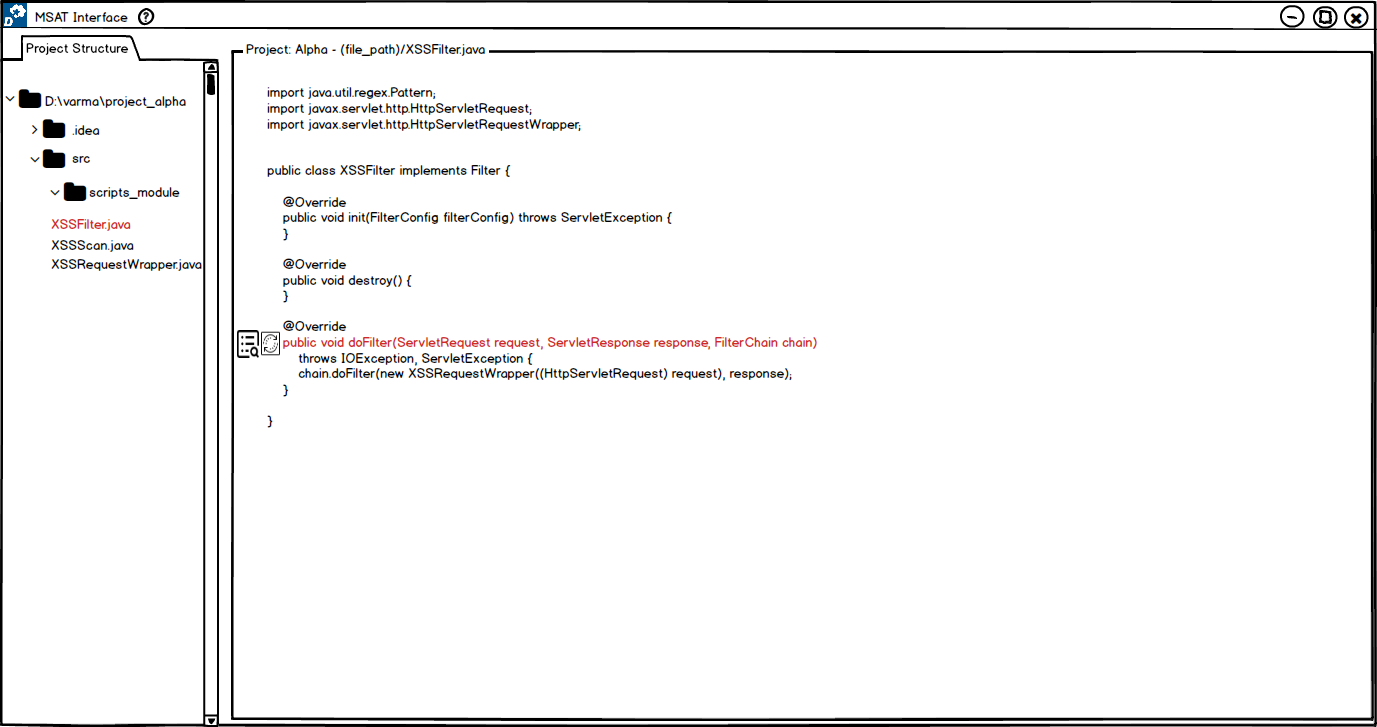
\includegraphics[width=\linewidth]{figures/solution_ideas_snaps/S21_multiple_icons}
	\caption{An interface prototype showing ‘multiple icons’ solution idea.}
	\label{fig:S21_multiple_icons}
\end{figure}

\textbf{Task – Success Criteria}: \\

On two clicks with different tool icons know that the bug is “Anti cross-site scripting filter”. The answer for number of tools is 2. \\

\textbf{Evaluation}: \\

Quantitative Results: \\

There are seven user study participants. All users had managed to perform the given task. This evaluation shows that the task success rate is 100 per cent. \\

Among the seven users, two users felt this is convenient in considering a final solution idea in showing the analysis results, in comparison to other solution ideas. In terms of usability on a scale of 0 to 10, where 0 being the worst and ten being the best, seven users rated the solution idea as 5,8,5,8,8,10, and 9, which averages to 7.57. \\

Qualitative Results: \\

Let us now investigate the reasoning behind the user’s choice of solution idea and respective ratings. User felt that separate icons is better to have in single glance but if more tools, then single standard icon is best in terms of scalability. Others mentioned that it overcrowds quickly if more than two gutter icons per row, it does not look pretty good having all icons in one place. One user suggested to have tool icons at project structure besides filename. One exciting aspect is that one user at first did not understand the icons, and later he clicked on icons and then understood the concept without the designer interference. \\

\textbf{Solution Idea – Single Icon}: \\

Once we have analysis results from the integrated tools, the interface shows respective bug findings in code editor. In the present scenario, interface shows a single icon in the gutter at the respective line of code where the tool identifies the bug no matter which tool has identified it. A text box which is a popup on click of the standard icon shows the details about which tool identified it as a bug. This idea could be well understood, looking at following \autoref{fig:S21_single_icon} or a complete prototype images added in appendix. \\

\begin{figure}[hbt!]
	\centering
	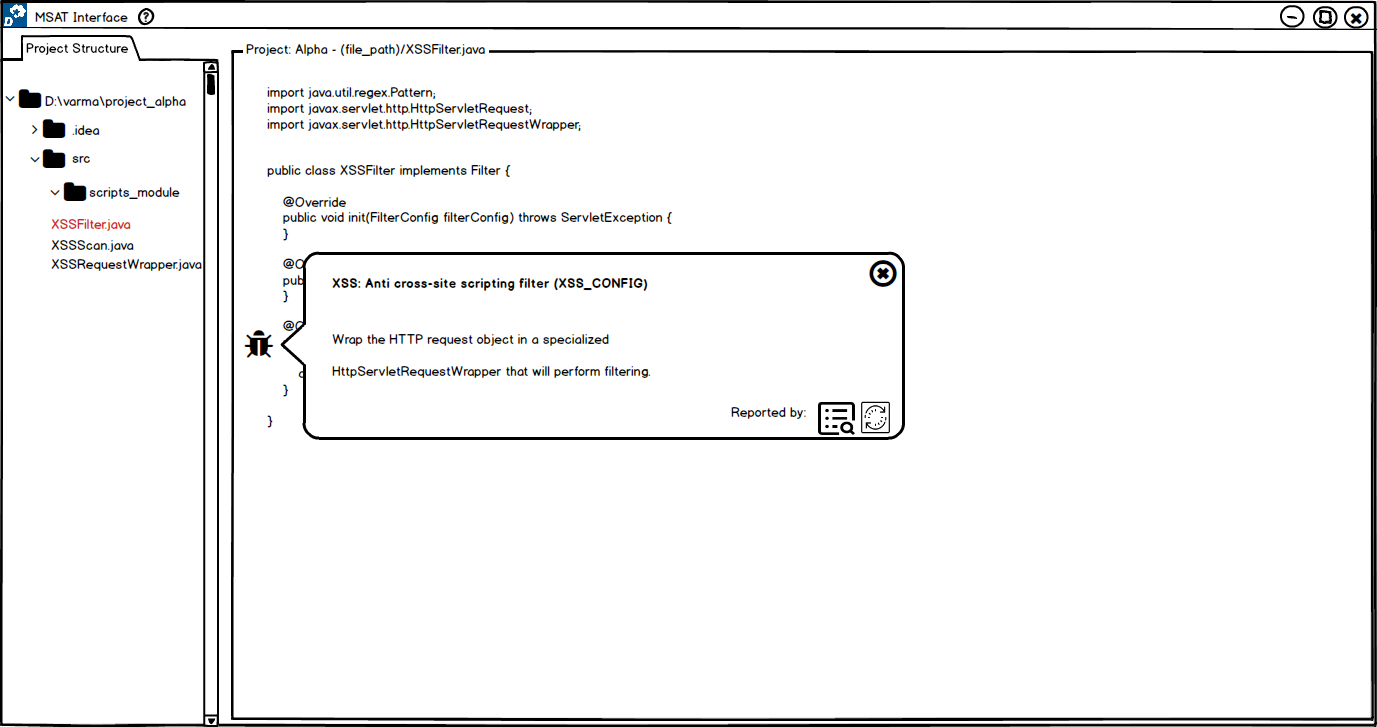
\includegraphics[width=\linewidth]{figures/solution_ideas_snaps/S21_single_icon}
	\caption{An interface prototype showing ‘single icon’ solution idea.}
	\label{fig:S21_single_icon}
\end{figure}

\textbf{Task – Success Criteria}: \\

On single click on bug icon know that the bug is “Anti-cross-site scripting filter”. The answer for number of tools is 2. \\

\textbf{Evaluation}: \\

Quantitative Results: \\

There are seven user study participants. All users had managed to perform the given task. This evaluation shows that the task success rate is 100 per cent. \\

Among the seven users, five users felt this is convenient in considering a final solution idea in showing the analysis results, in comparison to other solution ideas. In terms of usability on a scale of 0 to 10, where 0 being the worst and ten being the best, seven users rated the solution idea as 7,7,6,10,10,9, and 10, which averages to 8.43. \\

Qualitative Results: \\

Let us now investigate the reasoning behind the user’s choice of solution idea and respective ratings. Users said as a developer, the vital aspect is to find bug but not which tool reported it. Having a single icon is better in terms of readability, more straightforward, more convenient as it does not overcrowd the left-side gutter and looks much better. A couple of suggestions from users are to also add tool name instead of tool icon for general user to understand quickly and other user says in similar context that to have a popup for icons to know the respective tool names. One additional improvisation request is to have some bug severity representation at gutter section. \\

\begin{myboxi}{{\textbf{RQ 1-3: From code view perspective, will single icon suffice the showing of different tools icons?}}}
\\ \\ Single icon solution idea outwins multiple icons solution idea with a majority of 5 out of 7 users. 
\end{myboxi}


\subsubsection{RQ 2: What feedback works to know that the bug fixing is on-going?}

As part of this primary research question, we are going to first evaluate the three feedback mechanisms proposed in context of analysis view, i.e., animated icons, progress bar and pending status popup in our designed MSAT-UI ( Multiple Static Analysis Tools – User Interface ) and later in context of code view with other solution ideas. \\

The ‘animated icons’ solution idea demonstrates that when the user selected a bug finding and attempted to fix it by submitting for re-analysis, interface shows a feedback with respective tool icons with animation for that bug which is under analysis. This idea could be well understood, looking at following \autoref{fig:S22_animation} or a complete prototype images added in appendix.  \\ \\


\begin{figure}[hbt!]
	\centering
	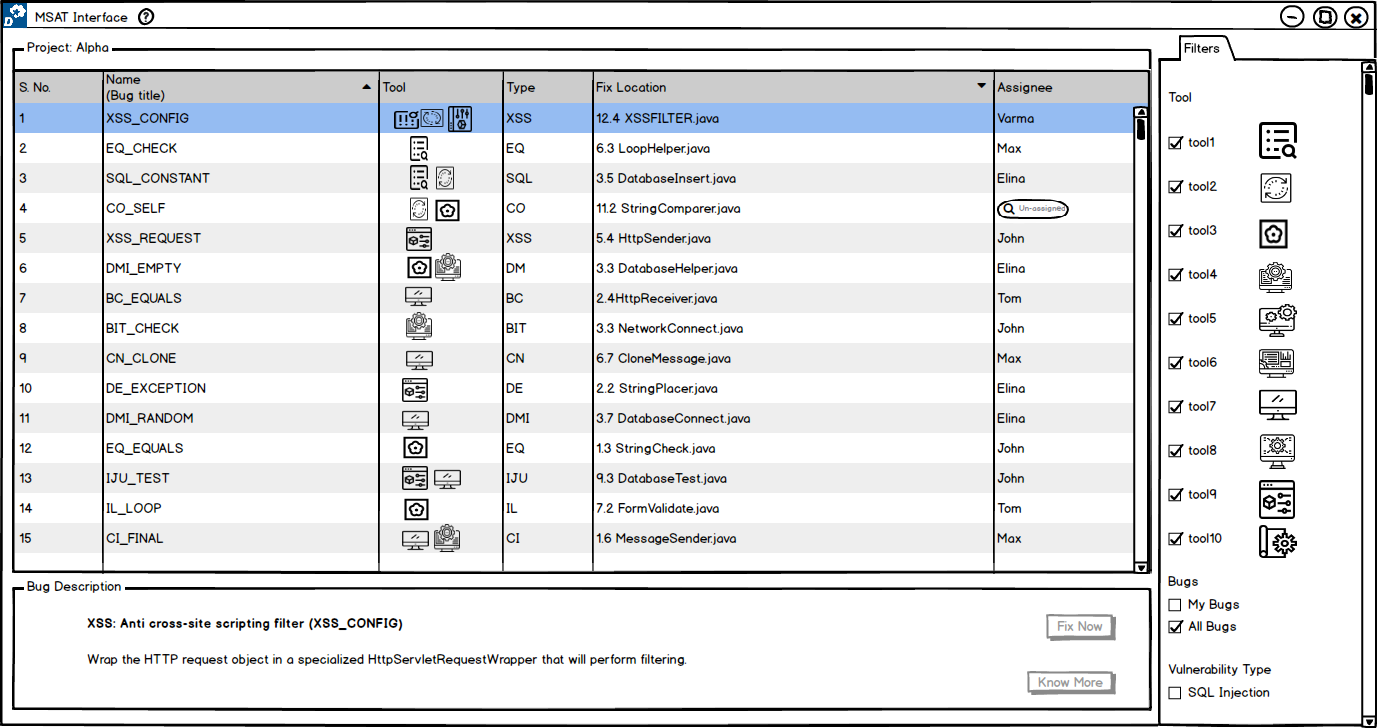
\includegraphics[width=\linewidth]{figures/solution_ideas_snaps/S22_animation}
	\caption{An interface prototype showing ‘animated icons’.}
	\label{fig:S22_animation}
\end{figure}


Next, the “progress bar” solution idea is demonstrated as when a user works on a bug and submitted for analysis. Then the interface shows progress bars as feedback with how far the tools finishes analysing. It shows progress bars for one or many tools that found that particular bug. This feedback is displayed when clicked on the bug, which is under analysis. Also, the respective icons are shown as blurred, indicating they are under analysis in contrast to previous solution idea. This idea could be well understood, looking at following \autoref{fig:S22_progress} or a complete prototype images added in appendix.  \\ \\


\begin{figure}[hbt!]
	\centering
	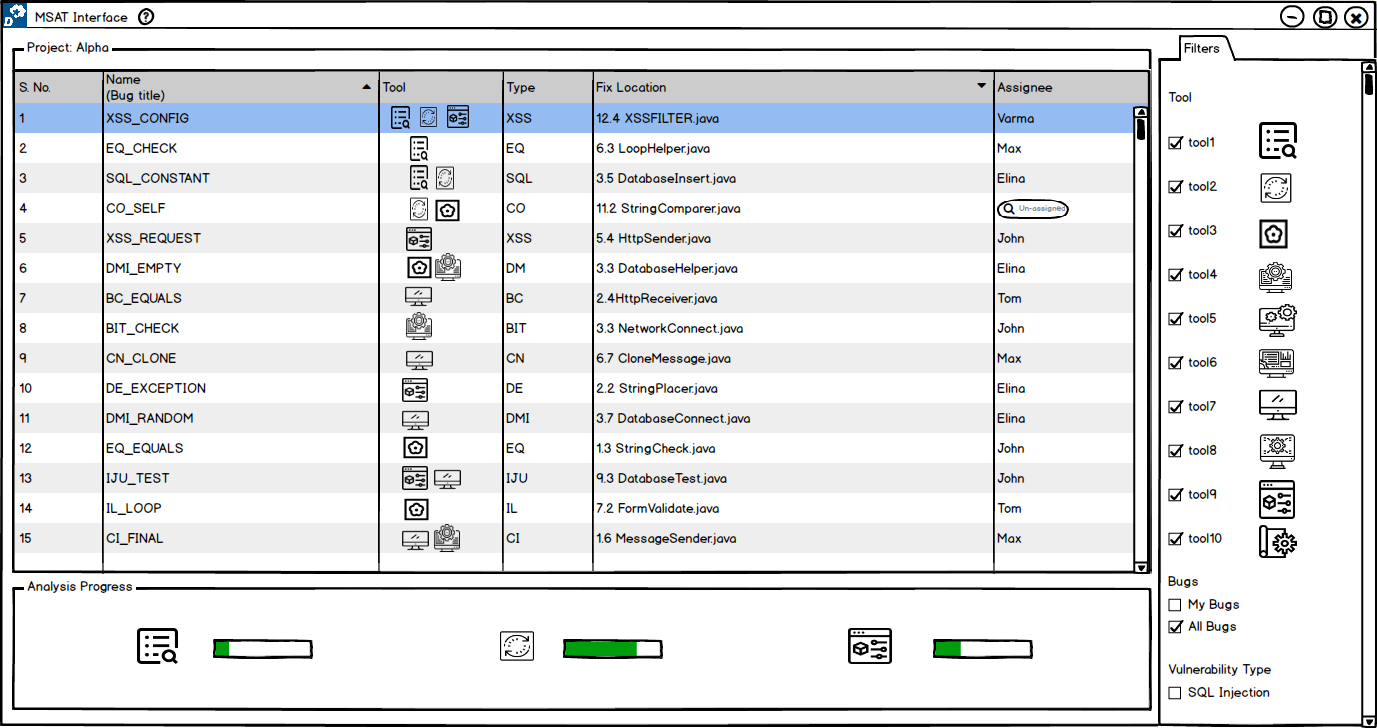
\includegraphics[width=\linewidth]{figures/solution_ideas_snaps/S22_progress}
	\caption{An interface prototype showing ‘progress bar’.}
	\label{fig:S22_progress}
\end{figure}


So finally, the third solution idea, i.e., “pending status popup” demonstrates the textual feedback about what the analysis tools are scanning as an example, tool name, timestamp, respective filename with code under analysis. On click of text link named “pending” in the status column in the given table view, it displays the popup. This idea could be well understood, looking at following \autoref{fig:S22_popup} or a complete prototype images added in appendix. \\ \\


\begin{figure}[hbt!]
	\centering
	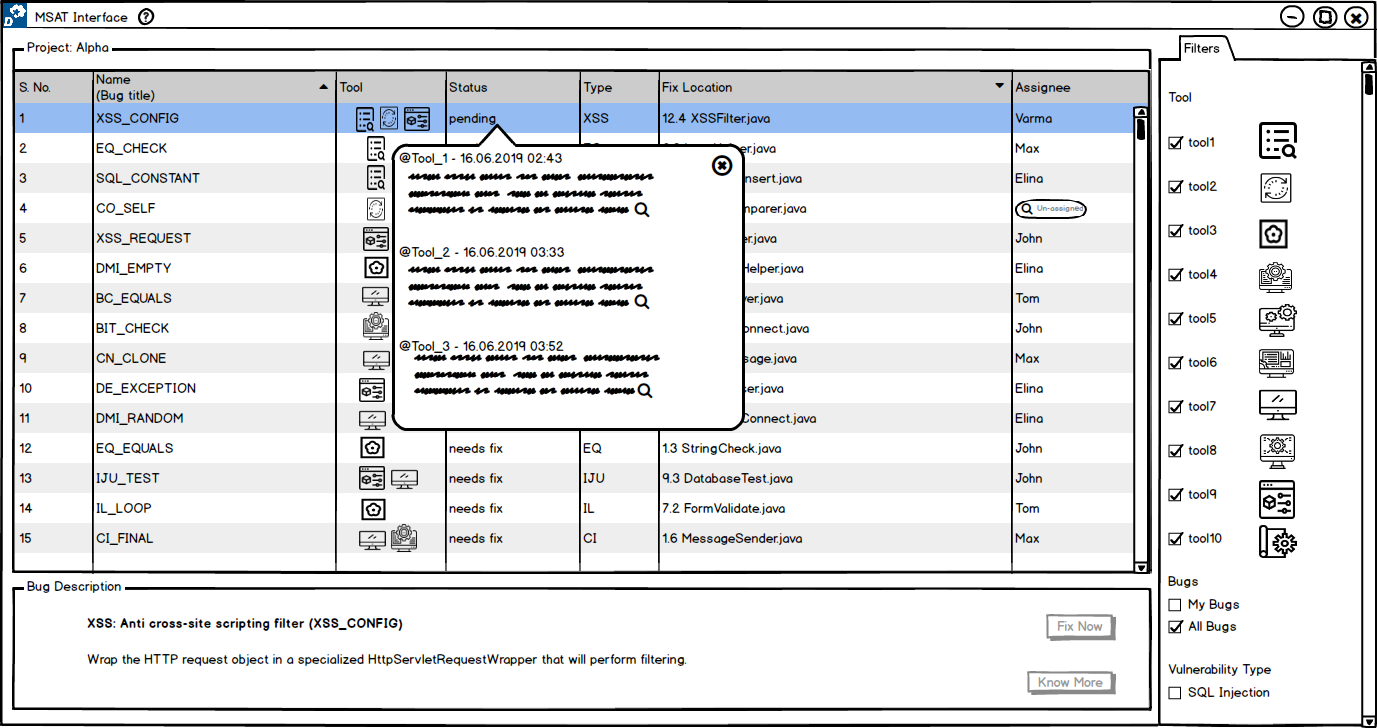
\includegraphics[width=\linewidth]{figures/solution_ideas_snaps/S22_popup}
	\caption{An interface prototype showing ‘pending status popup’.}
	\label{fig:S22_popup}
\end{figure}

The User Scenario, Tasks, and Follow up questionnaire is similar to previous research question. However, the tasks are demonstrated by the designer in order to make the user understands the feedback mechanism ideas. The reason for not doing so is the limitation with prototype builder, i.e., Balsamiq not having dynamic nature in showing animation effects and thereby designer tries to mock the animation effect with multiple clicks which could be tedious if asked the user to do. \\ \\

\textbf{User Scenario}: \\

Assume that the user worked on a bug and changed some code related to it. Next, submitted bug fix code for analysis. \\ \\

\textbf{Task}: \\

Observe what happens after clicking on “Fixed” button. \\

\textbf{Follow Up}: \\

\begin{enumerate}
\item Among the solution, ideas presented, which one does the user feel convenient (easy to use) with for the given task?
\item Why is it the mentioned solution idea is convenient?
\item How do the user rate in terms of perceived usability ranging from O, be lower to 10, be high for provided solution designs in comparison?
\end{enumerate}

\textbf{Evaluation}: \\

Quantitative Results: \\

Since the designer has performed the tasks, there is no such as task success as seen in previous research question. Among the seven users, no user felt any solution idea is not convenient in comparison to other solution ideas to be considered as final solution idea in showing as a feedback during the bug fixing process.  Most users preferred them to have in combinations and especially three users explicitly felt status pending with pop up would be more useful. Nevertheless, users appreciated each feedback in the context of its respective usage scenario. In terms of usability on scale of 0 to 10, where 0 being worst and 10 being the best, 7 users rated “animated icons” solution idea as 7,7,6,8,8,7 and 8 which averages to 7.28, “progress bar” solution idea as 7,8,8,10,9,8 and 6 which averages to 8 and finally “pending status popup” solution idea as 4,8,8,7,8,9 and 10 which averages to 7.7. \\

Qualitative Results: \\

Let us now investigate the reasoning behind the user’s choice of solution idea and respective ratings. For animated icons, one user explicitly stated that it is useful to know what the tool is analysing. For progress bar, one user says as the optimised tools, in general, takes less time and thereby it has no priority as it also kind of fancy in his perspective. For status pending pop up, the user expressed his interest in knowing what is happening, and this feedback helps so. Others also mentioned that it is much convenient,  this feedback is solely enough, it is more detailed, having timestamp when it is processed it is good. Overall, the users requested to merge the feedbacks. In a sense, to have them all in a proposed prototype. Each one helps in its way of knowing what the tool analyses, how far the tool analysis a bug and more important details of the analysis in third feedback. Also, one user suggested to merge both code editor view and analysis viewer in the same window. \\

\begin{myboxi}{{\textbf{RQ 2-1: When submitting the bug for analysis, what feedback does user feel convenient among animation, progress bar or popup?}}}
\\ \\	Each has its prominence. However, users felt that pending status is more useful among them.
\end{myboxi}

\begin{myboxi}{{\textbf{RQ 2-2: Does a single type of feedback suffice or requires combination?}}}
\\ \\	Users felt the requirement of the combination of all feedbacks as each serve in its scope.
\end{myboxi}

Let us now look into the solution ideas for Code view perspective. The proposed solution ideas are, namely ‘alerts’ and ‘status spinner.’ \\


The “alerts” solution idea demonstrates that when a user has submitted a bug for analysis, and later he if off the analysis screen and probably working on a different task. In this scenario,  the interface shows a popup whether the bug fix got succeed or not as feedback. It also has two call to action buttons such as “try again” or “ok”. The “try again” action button help to work on the same bug again and so this button could link to the program file where the user made previous changes concerning the bug finding. This idea could be well understood, looking at following \autoref{fig:S22_try_again_alert} or a complete prototype images added in appendix. \\


\begin{figure}[hbt!]
	\centering
	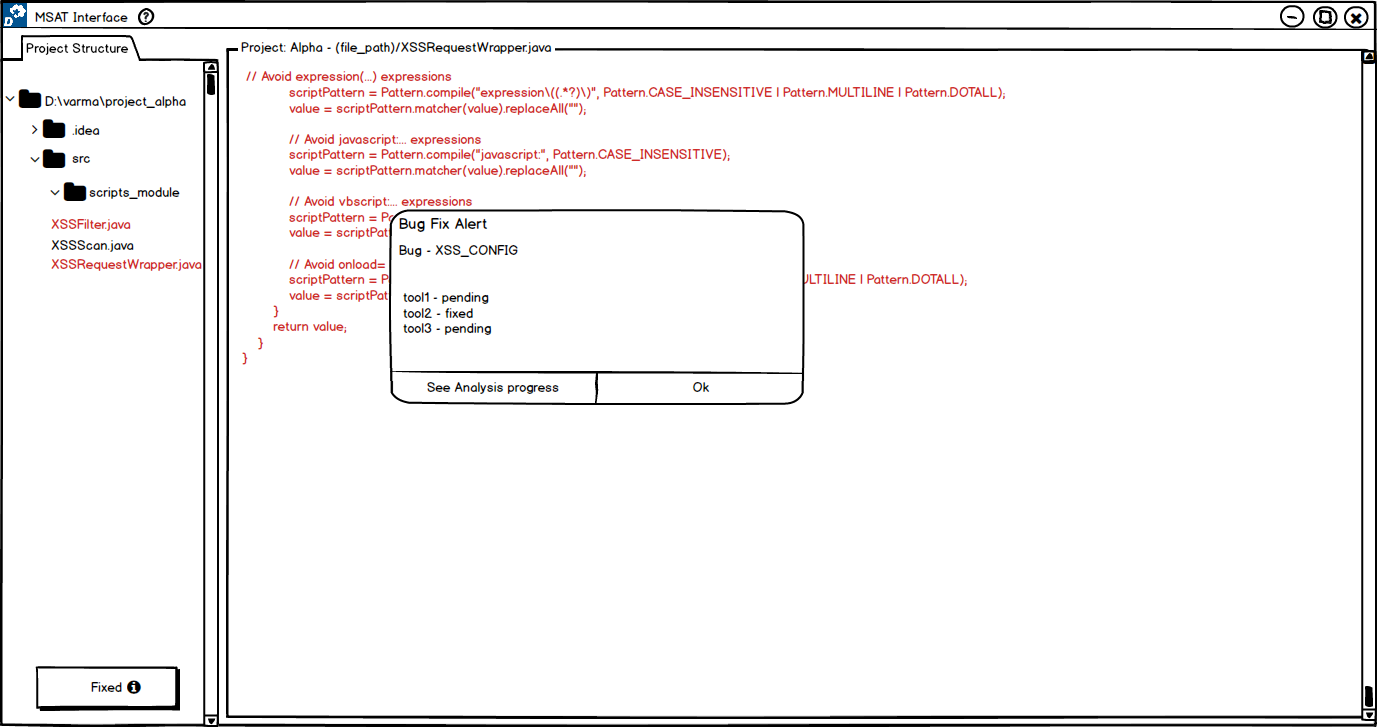
\includegraphics[width=\linewidth]{figures/solution_ideas_snaps/S22_try_again_alert}
	\caption{An interface prototype showing ‘alert’.}
	\label{fig:S22_try_again_alert}
\end{figure}

The “status spinner” solution idea demonstrates that when a user has submitted a bug for analysis, and later he is off the analysis screen and probably working on a different task. In this scenario, the user interface shows a feedback at the corner of the screen with a busy indicator like spinner. This idea could be well understood, looking at following \autoref{fig:S22_status} or a complete prototype images added in appendix. This approach indicates whether an analysis is running in the background or not. \\


\begin{figure}[hbt!]
	\centering
	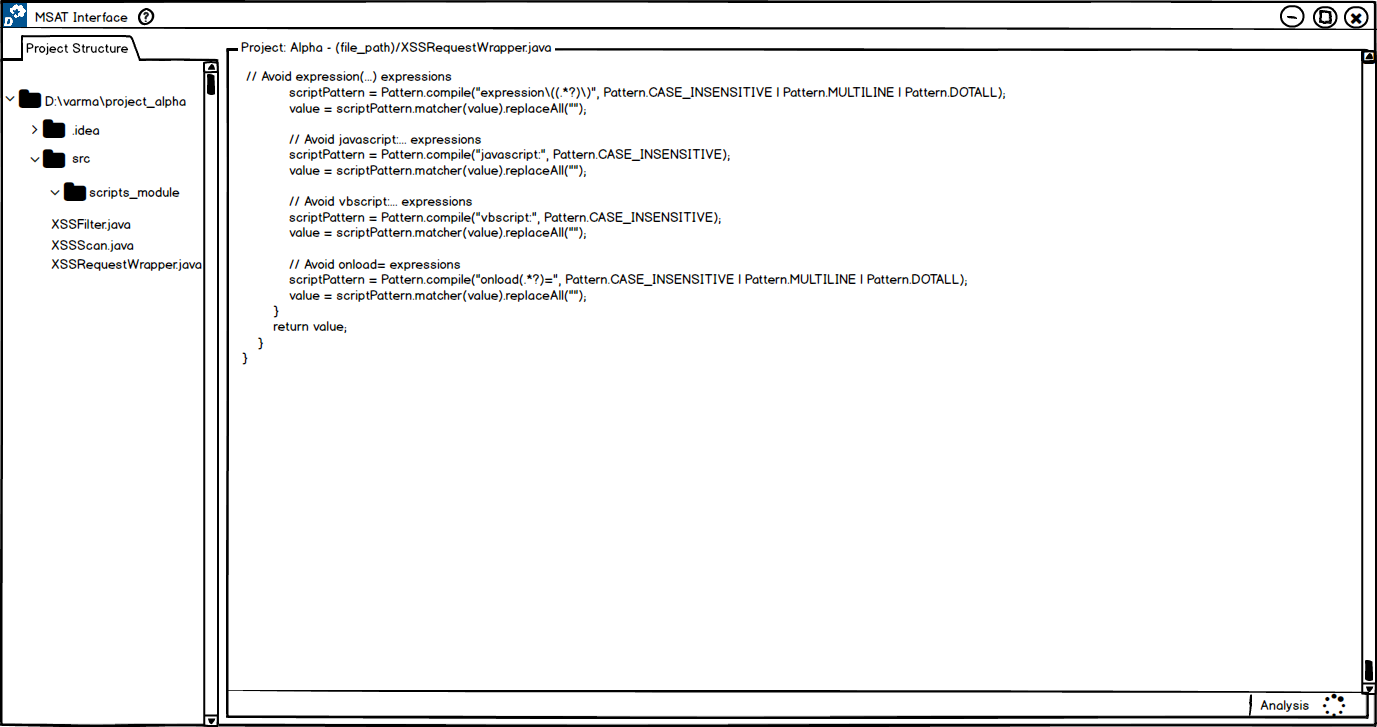
\includegraphics[width=\linewidth]{figures/solution_ideas_snaps/S22_status}
	\caption{An interface prototype showing ‘status spinner’.}
	\label{fig:S22_status}
\end{figure}

Next, we examine the following User Scenario, Task and Follow up questionnaire protocol. \\

\textbf{User Scenario}: \\

In addition to the previous scenario, after submitting code for analysis, instead of being on the bug results window, the user moved on to the next task in code editor. \\

\textbf{Task}: \\

Observe the visuals with alert box and status bar with spinner as demo. \\

\textbf{Follow up}: \\

\begin{enumerate}
\item Among the solution, ideas presented, which one does the user feel convenient (easy to use) with for the given task?
\item Why is it the mentioned solution idea is convenient?
\item How do the user rate in terms of perceived usability ranging from O, be lower to 10, be high for provided solution designs in comparison?
\item Would the user prefer having multiple feedbacks?
\end{enumerate}

\textbf{Evaluation}: \\

Quantitative Results: \\

Since the designer has performed the tasks, there is no such as task success as seen in previous research question. Among the seven users, four users felt it “alerts” is convenient in comparison to other solution ideas to, as final solution idea in showing as a feedback during the bug fixing process. In terms of usability on scale of 0 to 10, where 0 is worst and ten being the best, seven users rated “status spinner” solution idea as 6,8,6,10,6,9 and 8 which averages to 7.57 and for “alert” solution idea as 2,8,8,8,9,9 and 9 which averages to 7.57. \\

Qualitative Results: \\

Let us now investigate the reasoning behind the user’s choice of solution idea and respective ratings. In the context of status spinner, users felt that it is simple; if the user want to know status, then click on analysis. In the context of alerts, a couple of users felt it is annoying, not useful while working on different priority work and also takes them out of context their mind was he in. Nevertheless, there are positive opinions from other users saying that it draws positive attention, it shows details, and it does not require much transitions to know the status. There is one suggestion from his expertise background in coding that if we need to implement alerts, it is better to have in the context of bug fix failure. But not in success as the tool does not need to say it as fixed, as developer is already in the mindset that he fixed the bug before submitting to analysis. This mindset shows that this user is usually confident about his bug fixes. Some users preferred to have both as they serve different purposes and indeed, they are both helpful feedbacks. \\

\begin{myboxi}{{\textbf{RQ 2-3: From code view perspective, i.e., once user fixed a bug and submitted for analysis and then off the analysis results screen, then is popup notifications with analysis progress information better to busy status (spinner)?}}}
\\ \\	Popup notifications solution idea outwins status spinner with majority of 4 out of 7. Although remaining said it is annoying, but if needs implemented they would prefer to have when bug fix fails.
\end{myboxi}

Let us switch to the final main question. \\ \\

\subsubsection{RQ 3: How to carry traceability of bug fixing?}

We evaluate the following sub research questions in this context. \\

\begin{enumerate}
\item In tracing, will the user need to know the changes made to fix a bug affecting the analysis of other tools?
\item Does adjective mapping ease the user to trace the changes made in code in terms of bugs existence?
\item From code view perspective, will the bug tool icons with before/after code help understand the user in easing to fix it?
\end{enumerate}

The first two questions correspond to analysis view, and the third corresponds to code view. The solution ideas tested are namely ‘numbers’ and ‘adjectives’ for analysis view and “before/after” for code view. Firstly, let us look at the analysis view solution ideas and see how users evaluated them. \\

Now the user is provided with the following User Scenario, Task and Follow up questionnaire once we present both prototypes. Each task has task success criteria which we mentioned along with respective solution idea below. \\


\textbf{User Scenario}: \\

The user has been working on some part of code to fix a bug in last few working days. Now the user would like to see how the changes (commits) you made are affecting the analysis results of other tools. \\

\textbf{Task}: \\

Watch the results of all tools and decide on best commit among last three to revert as to start from that point. \\

\textbf{Follow up}: \\

\begin{enumerate}
\item Among the two solution ideas presented, which one does the user feel convenient (easy to use) with for the given task?
\item Why is it the mentioned solution idea is convenient?
\item How do the user rate in terms of perceived usability ranging from O, be lower to 10, be high for provided solution designs in comparison?
\end{enumerate}

\textbf{Solution Idea – Numbers}: \\

This idea demonstrates as when respective commits are made to fix a particular bug. User interface shows the commit ids along with some metrics, i.e., numbers of new bugs introduced or got fixed by its respective change as determined by a tool. This idea could be well understood, looking at following \autoref{fig:S23_metrics} or a complete prototype images added in appendix. \\


\begin{figure}[hbt!]
	\centering
	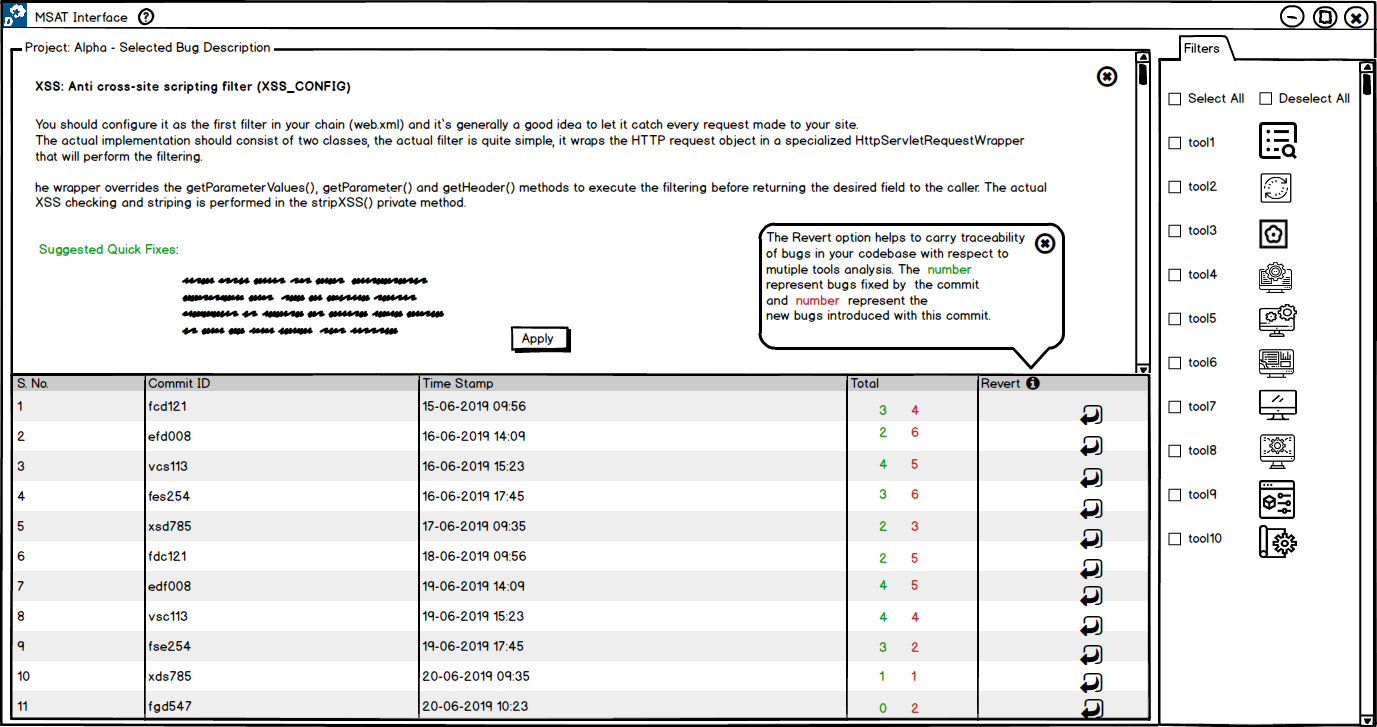
\includegraphics[width=\linewidth]{figures/solution_ideas_snaps/S23_metrics}
	\caption{An interface prototype showing ‘numbers’.}
	\label{fig:S23_metrics}
\end{figure}

\textbf{User Success Criteria}: \\

Selecting the commit id – fse254. \\

\textbf{Evaluation}: \\

Quantitative Results: \\

There are seven users participated in this user study. Out of which, five users can perform the task. This evaluation shows that the task success rate is 71.42 per cent. \\

Among the seven users, four users felt this is convenient in considering a final solution idea in showing the analysis results, in comparison to other solution ideas. In terms of usability on a scale of 0 to 10, where 0 is worst and 10 being the best, seven users rated the solution idea as 7,6,7,10,8,8 and 5, which averages to 7.28. \\

Qualitative Results: \\

Let us now investigate the reasoning behind the user’s choice of solution idea and respective ratings. Users felt it is incredibly complicated when he is unsure of what a number is. He tends to click on it as if it is a link, challenging to get to conclusion for the action needs to done in the context of the given task, it depends on the difficulty of the bugs represented in the numbers. Also, a couple of users suggested to have latest commits on the top as in terms of user consistency model, which we considered it as improvisation for prototype design in general. \\

\textbf{Solution Idea – Adjectives}: \\

This idea demonstrates as when respective commits are made to fix a particular bug. User interface shows the commit ids along with some adjective words, i.e., worst, bad, good, better and best. Each word demonstrates how easy or hard to fix the introduced bugs in general. As in previous solution idea, there could be a scenario where a change in specific commit could introduce new bugs or fix some bugs as reported by some tool. Now, in order to make it easy to evaluate or understand the numbers, adjectives could be used as a replacement. These adjectives are determined as rough time estimate difference to fix new bugs, and bugs got fixed. In practice, tools like Codacy show a rough time estimate. This idea could be well understood, looking at following \autoref{fig:S23_adjectives} or a complete prototype images added in appendix. \\


\begin{figure}[hbt!]
	\centering
	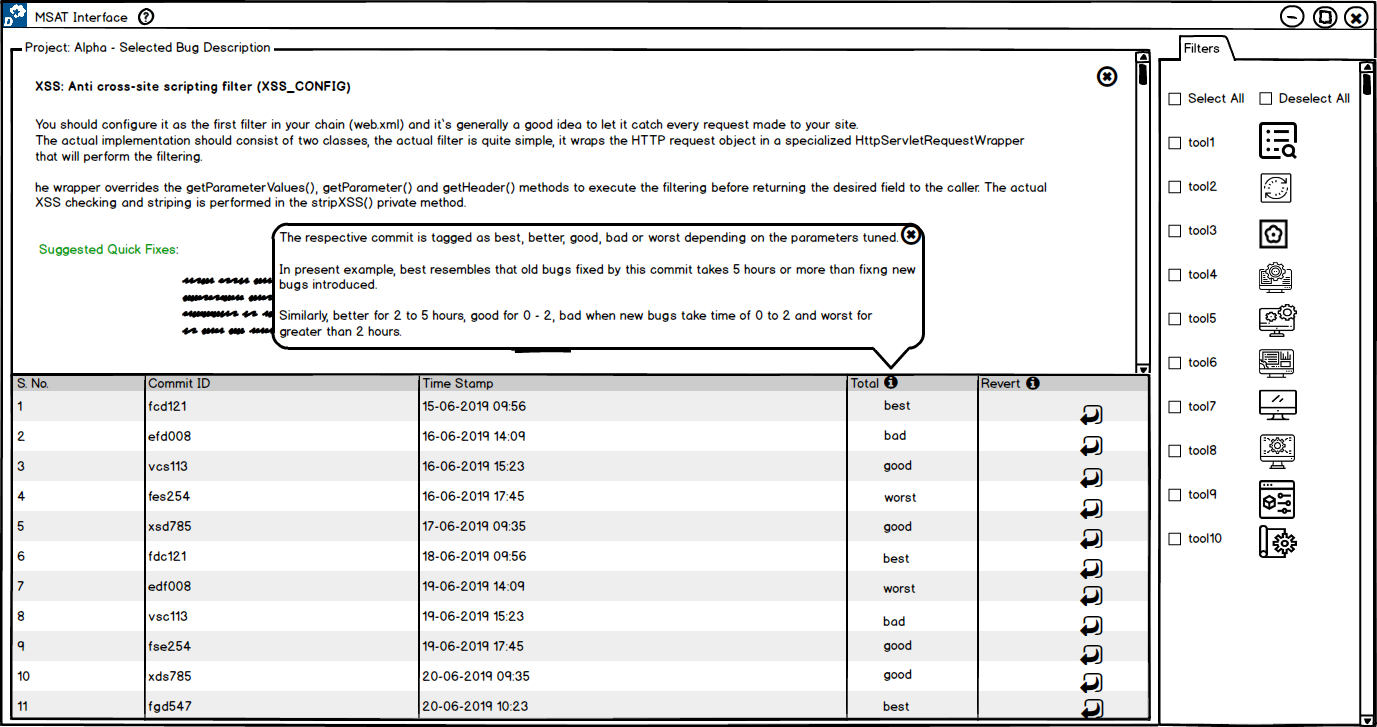
\includegraphics[width=\linewidth]{figures/solution_ideas_snaps/S23_adjectives}
	\caption{An interface prototype showing ‘adjectives’.}
	\label{fig:S23_adjectives}
\end{figure}

\textbf{User Success Criteria}: \\

Selecting the commit id – fgd547. \\

\textbf{Evaluation}: \\

Quantitative Results: \\

There are seven users participated in this user study. Out of which, six users can perform the task. This evaluation shows that the task success rate is 85.71 per cent. \\

Among the seven users, three users felt this is convenient in considering a final solution idea in showing the analysis results, in comparison to other solution ideas. In terms of usability on a scale of 0 to 10, where 0 is worst and 10 being the best, seven users rated the solution idea as 4,6,5,8,6,10 and 7, which averages to 6.57. \\

Qualitative Results: \\

Let us now investigate the reasoning behind the user’s choice of solution idea and respective ratings. Users felt that it depends on the expertise of the user, rough estimation of time is helpful and agreed to the scenario of having time estimate for this open research question. One user stated it is confusing, but all others accepted the idea. There are couple of suggestions such as combining this idea with previous one like numbers are shown at first and on click, shows what are those bugs whether good or bad in terms of fixing it in general and for beginners this idea is helpful. However, numbers are helpful for experts as time estimate could not be same among all colleagues in a software development team. One additional suggestion is to show what the tool reports as bugs and where. \\

\begin{myboxi}{{\textbf{RQ 3-1: In tracing, will the user need to know the changes made to fix a bug affecting the analysis of other tools?}}}
\\ \\ With number representation, it is good, but those do not represent difficulty.
\end{myboxi}

\begin{myboxi} {{\textbf{RQ 3-2: Does adjective mapping ease the user to trace the changes made in code in terms of bugs existence?}}}
\\ \\ It is helpful, especially for beginners.
\end{myboxi}
	
Now let us look into the solution idea in the context of code view, which we named it as “Before/After”. It shows two columns namely ‘Before’ and ‘After’ where ‘Before’ column has the code status before the commit happened while the bug is identified by a particular tool, wherein ‘After’ column, it shows the changes made to code. If the tool states as bug fixed, then it shows positive code change, and if the tool says it needs fix, then it determines the code where the bug is identified and at this point Before column shows the code before the change is made that lead to presence of bug. This idea could be well understood, looking at following \autoref{fig:S23_before_after} or a complete prototype images added in appendix. \\ \\


\begin{figure}[hbt!]
	\centering
	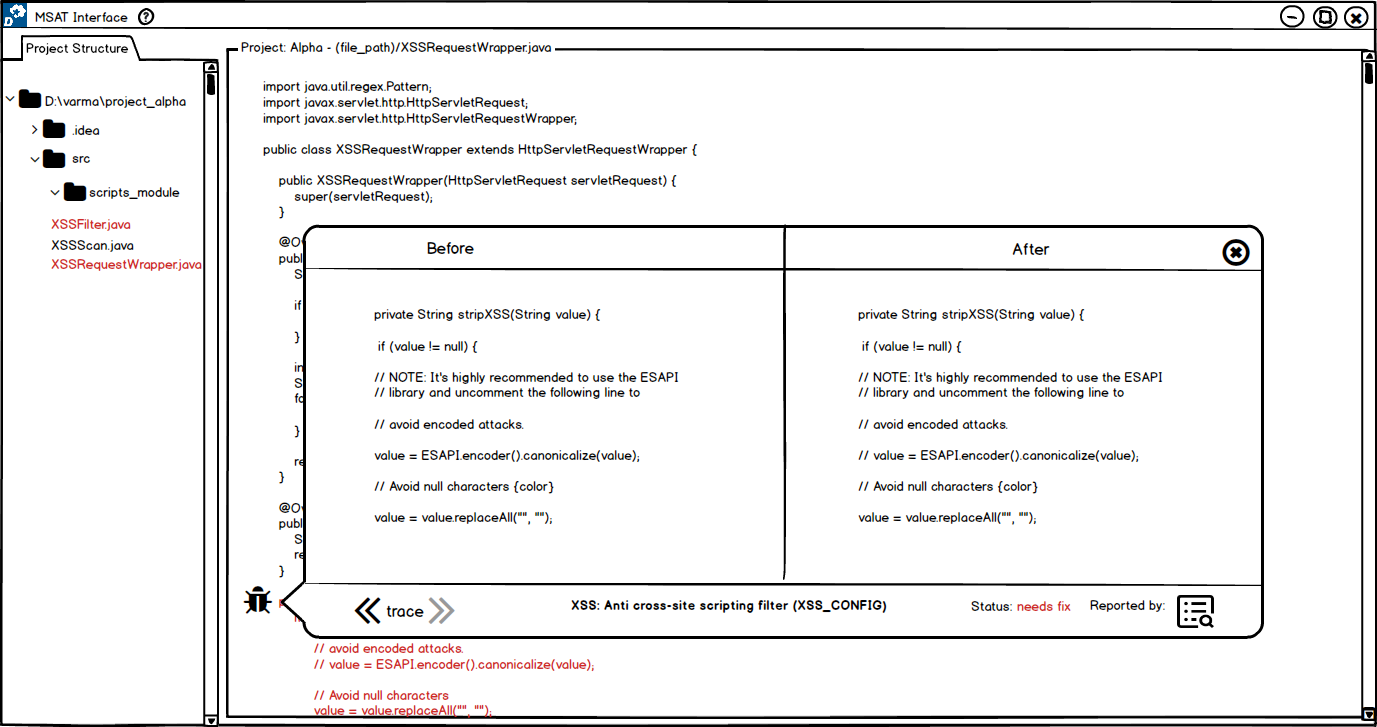
\includegraphics[width=\linewidth]{figures/solution_ideas_snaps/S23_before_after}
	\caption{An interface prototype showing ‘before/after’.}
	\label{fig:S23_before_after}
\end{figure}

The following User Scenario, Task and its Success Criteria and finally, a Follow-Up questionnaire is used to evaluate the design idea. \\

\textbf{User Scenario}: \\

As usual, the user is working on a code editor and notice a bug reported. The user remembers he has worked on this part of code before to fix some other bug. \\
 
\textbf{Task}: \\

Find out why the user changed the code before and plan to come up with better solutions that satisfies the tools reporting same part of code. In this case, what was the code line the user changed earlier to fix the bug reported earlier? \\

\textbf{Success Criteria}: \\

User finds that code line “ value = value.replaceAll("",""); ” is uncommented. \\

\clearpage
\textbf{Follow up}: \\

\begin{enumerate}
\item Do the user feel convenient by this UI with his workflow?
\item Why does the user think is the shown design is convenient or not so?
\end{enumerate}

\textbf{Evaluation}: \\

Quantitative Results: \\

There are seven users participated in this user study. Out of which, six users can perform the task. This evaluation shows that the task success rate is 85.71 per cent. Accordingly, users accepted the convenience with their usual workflow. \\

Qualitative Results: \\

Let us now investigate the reasoning behind the user’s choice of solution idea and respective ratings.  One user who was not able to do the task was he could not understand the user interface in first glance as it is novel. This only issue with one user could be considered as negligible and thereby proves the potential of the idea once design is clearly understood. \\

Users felt that this interface is more helpful than other views shown in analysis view solution ideas, helpful, novel, outstanding that user able to understand what changes he made, which all are positive. There are however few remarks and suggestions to make it more useful from user perspective such as having some background colour for changed line, colours for change in code, a single screen then no need of trace button. Still, however, the same user agreed with proposed design in the context of multiple tools. Other design idea for this scenario shared by the participant is Git like merge conflict design concept. Overall, users welcomed the design idea. One general suggestion is to have the flexibility of going to a code file on selection of a bug finding. \\


\begin{myboxi}{{\textbf{RQ 3-3: From code view perspective, will the bug tool icons with before/after code help understand the user in easing to fix it?}}}
\\ \\ Users felt helpful in tracing, although they did not understand the design in first glance as it is novel.
\end{myboxi}


\section{Summary}

During the UX cycle 2, there are seven users participated. The evaluation summarises answers for sub research questions as follows. The primary significant improvement over previous cycle to consider the enormous codebase and a code view perspective. For the first primary research question, i.e., display of analysis results, the solutions ideas are tested with a higher number of bugs and ten tools. From analysis view perspective, to answer whether separate list or single list help to identify the common bug, users felt the single list solution idea is more user-friendly and effortless to perceive. \\

In contrast, separate list solution idea offers no enough space to analyse appropriately and especially challenging while doing tasks like identifying the common bug reported by tools. Next, to answer whether the tags will help in scalability of bug results in comparison to separate list or single list, the users felt the UI to be novel and more open from design perspective. Still, however couple of developers stated it to be confusing. Thereby, a single list would still suffice in this scenario. Now from the code view perspective to answer will single icon suffice the showing of different tools icons, users have chosen single icon in majority, i.e., 5 out of 7 users. Users felt the vital aspect is about finding the bug but not who found it and moreover having separate icons would overcrowd the gutter space. \\

For the second primary research question, feedback, while bug fixing is on-going, to answer which feedback among animation, progress bar and popup are convenient as code base and number of tools scales. It still holds the same opinions as in previous UX cycle with new users in this cycle. The proposed feedbacks have their role of importance and so convenient to have in UI. Users felt pending status pop up solution idea to be more useful. Next, to answer does a single type of feedback suffice or requires combination, users felt the combination is needed as each has its importance within their scope.  Next from code perspective to answer, if popup notifications with analysis progress information better to busy status (spinner) in the scenario where user once fixed a bug and submitted for analysis and then off the analysis results screen. Among seven users, four users felt “alerts,” i.e., popup notifications is more convenient in choosing as final solution idea against the other. Couple of users felt alerts as annoying, but if we must implement it, then use it in case of bug fix failures as suggested by one user. \\

Finally, for the third primary research question, traceability of bug fixing, to answer that will the user need to know the changes made to fix a bug affecting the analysis of other tools. Evaluation results says that users felt its need but only having numbers could not depict the difficulty in fixing them. Further, to answer does adjective mapping ease the user to trace the changes made in code in terms of bugs existence, the time estimate with adjective mapping seems helpful for beginners. Still, the numbers would suffice for experts with a suggestion to show what the tool reports as bugs and where. Next, from code view perspective, to answer will the bug tool icons with before/after code help understand the user in easing to fix it. Although the users did not understand in first glance as the proposed user interface being novel, users felt it is more helpful in tracing. \\

\section{Lessons Learnt}

There are mainly a couple of limitations noticed during this user study process. They are: \\

\begin{enumerate}
\item Mockup screens jump to next screen without of scope click, i.e., when the user clicked on keyboard input or with random mouse clicks, results in jumping of mockup screens. We expect that mockup screens navigate when the user clicks the desired link or button.
\item Animation effects are not possible with available prototype builder, i.e., Balsamiq. \\
\end{enumerate}

As a workaround to overcome these limitations, we planned to have the mouse clicks in control to best possible and also to have additional mockups designed as back up. Next, we planned to demonstrate the effects of animation using multiple mockup screens. \\ \\

In this UX design cycle, we have tested the solution ideas of both analysis view and code view. It is found out the preferred solution designs of previous cycle still hold the same preference with new users after scaling both code base in terms of number of bug findings and the tools integrated to the codebase. Further, in the next UX design cycle, we planned to explore more scenarios for first primary research question, i.e., display, from code view perspective. Next, for the second primary research question, i.e., feedback, evaluate the proposed feedback ideas with existing tools having native user interfaces. Also, look into the 'alerts' solution idea, whether it is still acceptable with new users as it has mixed opinions. Finally, for the third primary research question, i.e., traceability, look into the scalability aspect of exiting ideas and also explore other solution ideas.